\renewcommand{\thepage}{\arabic{page}} \setcounter{page}{1}

\chapter{Properties of a Robot}

In this chapter the basic properties of the robot will be described, therefore the dynamic equations of the motor will be given and the behavior of the robot will examined with some basic simulations.

\section{Dynamic equation}
The robot arm, which can be seen in figure \ref{fig:robot}, has two joints within the same plain. 

\begin{figure}[h]
	\centering
	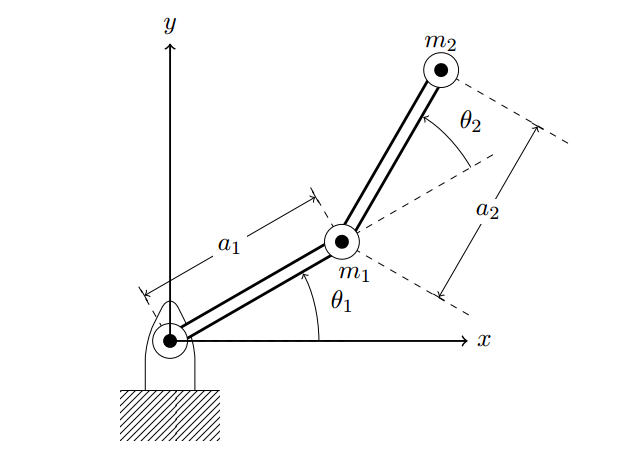
\includegraphics[width=0.85\textwidth]{pics/robot.png}\\
	\caption{Schmetics of the 2DOF Robot arm}
	\label{fig:robot}
\end{figure}

The basic differential equation of the robot can be seen by \eqref{eq:dynamic equation}.
\begin{gather}
\mathbf{\tau} = \mathbf{M}(\mathbf{q})\mathbf{\ddot{q}} + \mathbf{v}(\mathbf{q}, \mathbf{\dot{q}}) + \mathbf{g}(\mathbf{q}) + \mathbf{\tau}_D
\label{eq:dynamic equation}
\intertext{where:}
\begin{tabular}{>{$}l<{$} @{${}={}$} l}
\mathbf{\tau} & input torque vector \\
\mathbf{M}(\mathbf{q}) & inertia matrix\\
\mathbf{v}(\mathbf{q}, \mathbf{\dot{q}}) & centrifugal/corriolis vector\\
\mathbf{g}(\mathbf{q}) & gravitation vector\\
\mathbf{\tau}_D & disturbance vector
\end{tabular}\nonumber
\end{gather}

With the concept from Lagrange the dynamic equation of this system can be calculated:
\begin{align*}
\tau &= \left(\begin{array}{cc} {a_1}^2 m_1 + {a_1}^2 m_2 + {a_2}^2 m_2 + 2 a_1 a_2 m_2 \cos\!\left(q_2\right) & a_2 m_2 \left(a_2 + a_1 \cos\!\left(q_2\right)\right)\\ a_2 m_2 \left(a_2 + a_1 \cos\!\left(q_2\right)\right) & {a_2}^2 m_2 \end{array}\right)
\left(\begin{array}{c}
\ddot{q}_1\\ \ddot{q}_2
\end{array}\right) \\
&+ \left(\begin{array}{c} - a_1 a_2 m_2 \dot{q}_{2} \sin\!\left(q_2\right) \left(2 \dot{q}_{1} + \dot{q}_{2}\right)\\ a_1 a_2 m_2 {\dot{q}_{1}}^2 \sin\!\left(q_2\right) \end{array}\right)
\\
&+ \left(\begin{array}{c} g m_2 \left(a_2 \cos\!\left(q_1 + q_2\right) + a_1 \cos\!\left(q_1\right)\right) + a_1 g m_1 \cos\!\left(q_1\right)\\ a_2 g m_2 \cos\!\left(q_1 + q_2\right) \end{array}\right)

\end{align*}


\section{Simulation of the robot dynamics}

To check if the previous derived dynamic equations are reasonable, some basic simulations can be performed. In these simulations the robot arm will be taken into some specific initial conditions and the behavior will be simulated without any external force applied to the system.\\
There are three different initial conditions chosen. The first one is the robot arm points down and it rests in its stable equilibrium state. The next one is keeping the robot in its unstable equilibrium by pointing straight up. The last initial condition is an arbitrary setup, outside of the previous given equilibrium states.\\
In figure \ref{fig:stable} it can be seen that the robot arm is staying at rest and does not start to move. On one joint there can be some minor oscillation seen, which can be explained by the numerical error of the simulation.
\begin{figure}[]
	\centering
	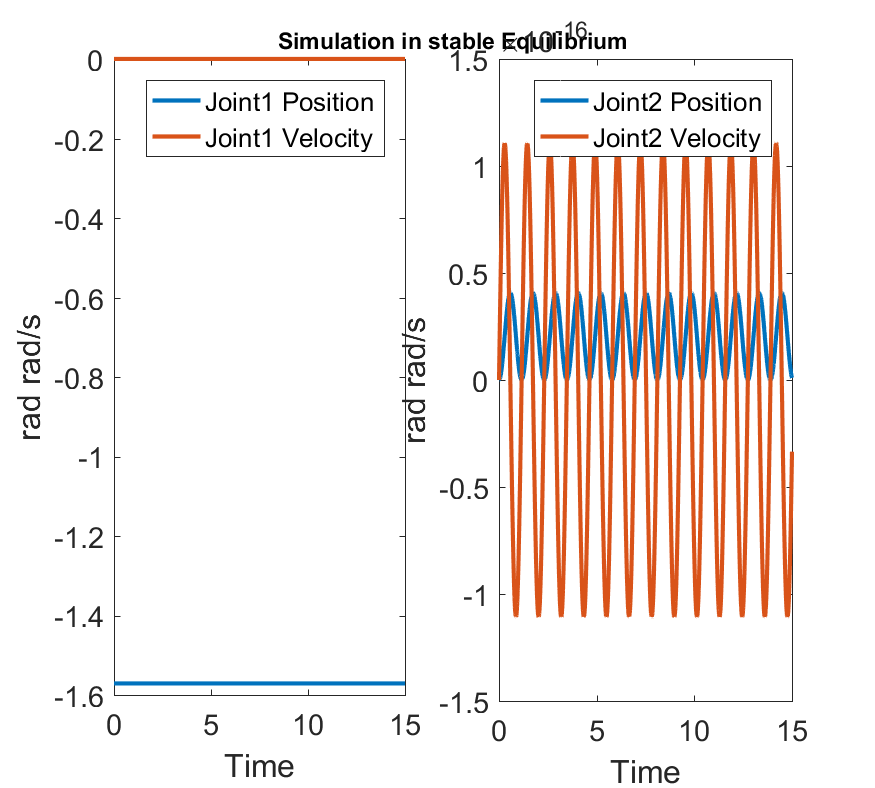
\includegraphics[width=0.60\textwidth]{pics/SimulationinstableEquilibrium.png}\\
	\caption{Simulation with initial condition in stable equilibrium}
	\label{fig:stable}
\end{figure}

The next simulation can be seen in figure \ref{fig:unstable}, here the initial condition of the robot arm was within the unstable equilibrium. Theoretically the robot will stay at rest within this state, unfortunately by some numerical error, caused by the simulation, the robot arm starts to move after around 7 seconds and continuous to swing with some chaotic pattern. Since the numerical error within the system gets integrated over time and there is no friction within the system, the movement of the robot is not expected to stop in anytime.
\begin{figure}[]
	\centering
	\includegraphics[width=0.60\textwidth]{pics/SimulationinunstableEquilibrium.png}\\
	\caption{Simulation with initial condition in unstable equilibrium}
	\label{fig:unstable}
\end{figure}

The last simulation is the initial condition outside of any equilibrium and the movement of all joints are expected to take place immediately; in comparison to the last simulation, which take 7 seconds to start moving visibly. The results of the simulation can seen in figure \ref{fig:outside}. The joints move in a chaotic way, as it has been expected.
\begin{figure}[]
	\centering
	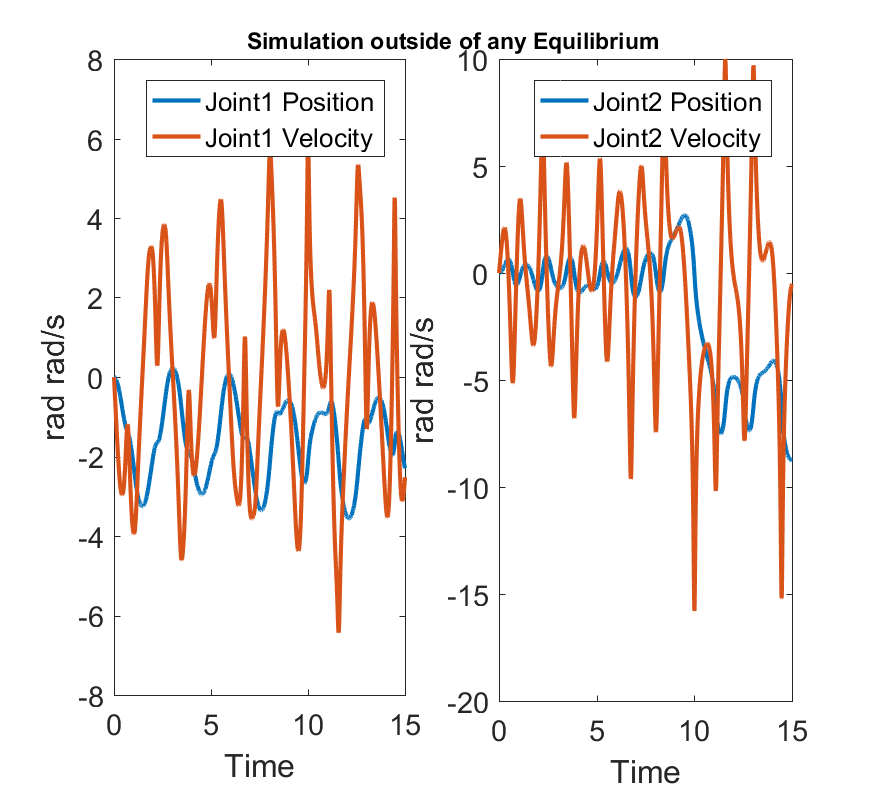
\includegraphics[width=0.60\textwidth]{pics/Simulationoutsideofanyequilibrium.png}\\
	\caption{Simulation with initial condition outside of any equilibrium}
	\label{fig:outside}
\end{figure}

All results of the simulations show expected behavior and we can assume that the model, which has been used, is correct.
